In contrast to wide-field microscopy, a confocal microscope illuminates only a small part of the object under investigation. Thereby, background noise is suppressed, and resolution is increased \cite{Lakowicz2006}. In this thesis, molecules dissolved in a solution are examined. Here, confocal fluorescence microscopy allows the detection of single molecules, which is essential for the understanding of biological processes, as discussed in Chapter~\ref{Chapter:Introduction}. 

First, this section presents the setup and the functionality of the used confocal fluorescence microscope. After that, in Section~\ref{Section:Measurements}, the procedure for measurements, and the format of the recorded data is discussed. 

\subsection{Setup}

A sketch of the used confocal fluorescence microscope can be found in Figure~\ref{fig:Setup}. The objective focuses the red and blue laser beams on a small part of the solution containing the investigated samples. The samples are either intrinsic fluorophores or dye-labeled molecules that can be excited by the incoming laser light. Since the emitted fluorescence light is Stokes shifted, it can pass the dichroic mirror, while back-scattered laser light is deflected. The fluorescence light is focused on a pinhole. Thereby, it is ensured that only light from the focus of the objective is transmitted. Another dichroic mirror separates the red and blue fluorescence light.  There is a detector for each color of fluorescence. For the detectors, avalanche photodiodes (APDs) were used because they offer photon detection efficiencies at around \SI{70}{\percent} and a time resolution down to \SI{350}{\pico\second} \cite{CountT,tauSPAD}. Therefore, they allow the counting of single photons, which is essential for \gls{BTCCD}, see Section~\ref{Section:BTCCD}.

\begin{figure}[h!]
	\centering
	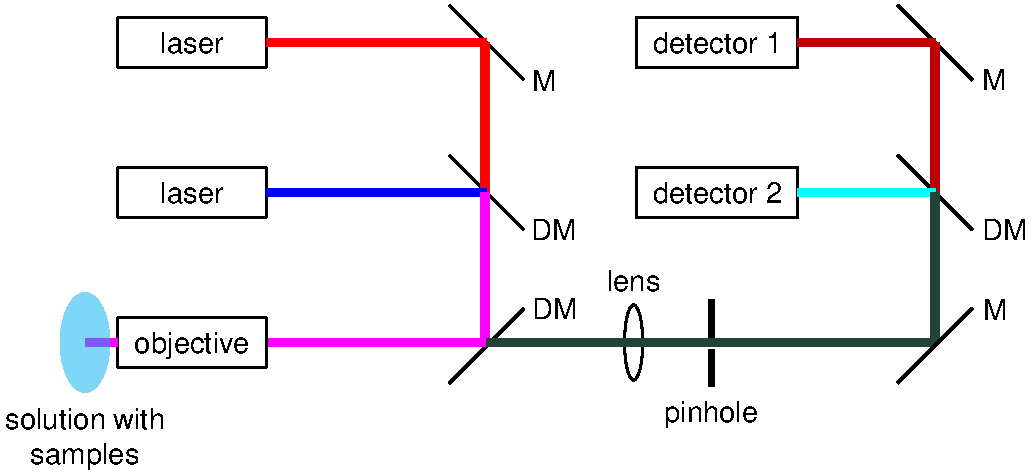
\includegraphics[width = 13cm]{Setup.pdf}
	\caption[Sketch of used confocal fluorescence microscope]{Sketch of the used confocal fluorescence microscope \cite{MicroTime200,Schwille2001}. (D)M stands for (dichroic) mirror.}
	\label{fig:Setup}
\end{figure}

The combination of objective, shape of the incoming laser beam, and pinhole leads to a spatial distribution of the fluorescence intensity in the sample solution, the so-called confocal detection volume. It can be described by a three-dimensional Gaussian
\begin{equation} \label{Equation:3DGaussian}
	I(x, y, z) = I_0 \cdot \exp\left( -2 \frac{x^2+y^2}{r_0^2}\right) \cdot \exp\left(-2 \frac{z^2}{z_0^2}\right),
\end{equation}
where the $xy$-plane is perpendicular to the direction of the incoming laser beam and $I_0$ is the peak intensity. Using the parameters $r_0$ and $z_0$, an effective volume 
\begin{equation} \label{Equation:DefinitionConfocalVolume}
	V_{eff} = \pi^{3/2} \cdot r_0^2 \cdot z_0
\end{equation}
can be defined \cite{Schwille2001}. Since $r_0$ and $z_0$ depend on the properties of the objective and the wavelength, the confocal detection volumes are different for both colors. The shorter wavelength of the blue laser leads to a smaller confocal detection volume compared to the red channel. The properties of the objective depend on the wavelength, and lead to a relative shift of both volumes, see Figure~\ref{fig:ConfocalVolumeTrajectories}. 

For all measurements with the confocal fluorescence microscope, first, the focus of the objective was set on the surface of the cover glass. Then, it was raised by \SI{10}{\micro\meter} into the solution. Thereby, it is ensured that molecules that stick to the cover glass do not disturb the measurement.

\subsection{Measurements} \label{Section:Measurements}

Each laser was operated at a frequency of \SI{10}{\mega\hertz}. Therefore, a laser pulse of the same color was emitted every \SI{100}{\nano\second}. The two lasers together were used alternating. This means that the time difference between the emission of a red and a blue laser pulse was set to \SI{50}{\nano\second}. This excitation scheme is called \glsfirst{PIE}. Since only one laser is powering at a time, its main advantage is the reduction of spectral cross-talk caused by non-ideal optical elements in the setup such as dichroic mirrors \cite{Mueller2005}.\\

A measurement with the confocal fluorescence microscope consists of the detection of photons by the detectors in a certain measurement time $T$. For each detected photon, three parameters are saved:
\begin{itemize}
	\item channel number: number of the detector that recorded the photon
	\item micro time $\tau$: time difference between the photon detection and the last red laser pulse 
	\item macro time $t$: absolute time of the photon detection
\end{itemize}
Figure~\ref{fig:MeasurementData} visualizes the difference between micro time and macro time, as well as the format of the recorded data. The result of every measurement with the confocal fluorescence microscope is a list of detected photons containing the three information above. Diverse evaluation methods of the measured data have been proposed \cite{Wahl}. In this thesis, the methods \glsfirst{FCS} and \gls{BTCCD} are applied, further discussed in Sections~\ref{Section:FCS} and \ref{Section:BTCCD}. Both of them only use the channel number and the macro time while ignoring the micro time.

\begin{figure}[h!]
	\centering
	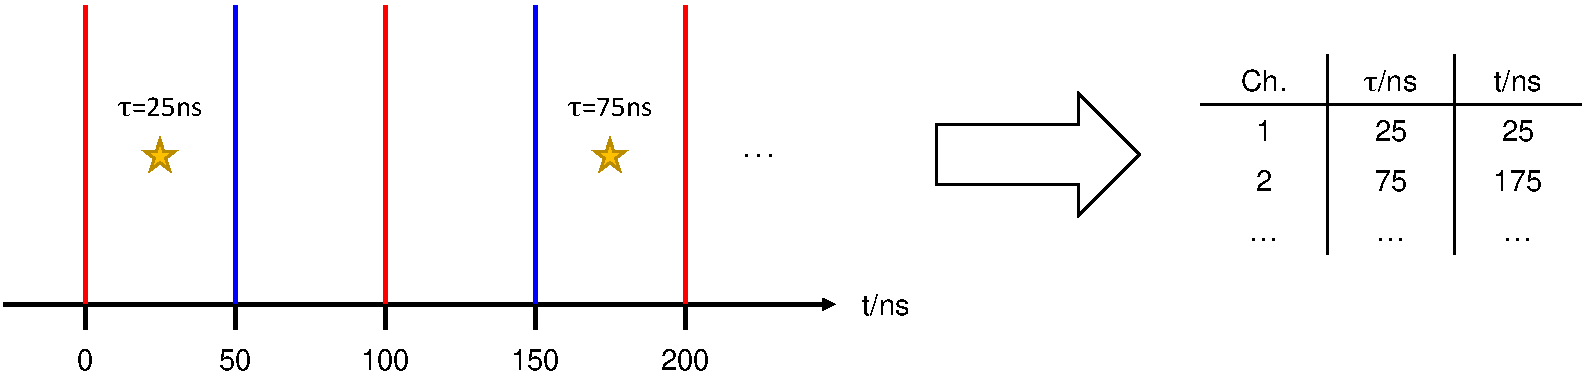
\includegraphics[width = \textwidth]{MeasurementData.pdf}
	\caption[Format of recorded measurement data]{Format of the recorded measurement data. The red and blue lines symbolize the laser pulses, whereas the yellow stars indicate the detection of a photon. For each photon, channel number, micro time $\tau$, and macro time $t$ are recorded.}
	\label{fig:MeasurementData}
\end{figure}